\section{System Description}
\subsection{}

\begin{frame}{Overview}

Three main components to system description:
\begin{itemize}
\item Register Files
\item Features
\item Instruction Sets
\end{itemize}

\end{frame}

\begin{frame}{Register File}

GenSim treats the register file as a set of flat memory regions (spaces)
with aliased `views'.

\end{frame}

\begin{frame}{Register File}

Three types of entry
\begin{itemize}
\item Slot - single, non banked register
\item Bank - `array' of values
\item Vector Bank - `array' of vector values
\end{itemize}

\end{frame}

\begin{frame}{Register File}

\centering
\only<1>{
	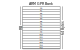
\includegraphics{figures/regbank-rb}
}

\only<2>{
	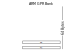
\includegraphics{figures/regbank-slots}
}

\end{frame}

\begin{frame}{Register File - Vectors}

\centering
\only<1>{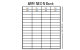
\includegraphics{figures/regbank-fp}}
\only<2>{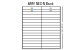
\includegraphics{figures/regbank-fp-dp}}
\only<3>{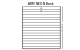
\includegraphics{figures/regbank-fp-q}}

\end{frame}

\begin{frame}{Features}

Primarily performance feature - give hints to simulator about things 
which change infrequently.

\end{frame}

\begin{frame}{Instruction Sets}

Which instruction sets are available to this architecture?

(Generally quite a short section)

\end{frame}
